\documentclass[week11]{csse2002}
\usepackage{slides}

\author{Brae Webb}

\title{CSSE2002 Week 11 Tutorial}
 
\begin{document}

\begin{frame}
\maketitle
\end{frame}

\begin{topic}{Admin}
\begin{enumerate}
	\item Tutor evaluations
    \item Assignment 3 is incoming --- good luck
    \item Assignment 2 marks are a while away
    \item Practicals and tutorials this week are useful for exams
\end{enumerate}
\end{topic}

\begin{topic}{This Week}
\begin{enumerate}
    \item Substitution Principle
    \item Class Extraction
\end{enumerate}
\end{topic}

\section{Substitution Principle}

\begin{topic}{Substitution Principle}
\framesubtitle{Review: Preconditions \& Postconditions}
\begin{subtopic}{1-}
A \highlight{precondition} restriction on the input to a method\\
A \highlight{postcondition} guarantee on the effect of a method
\end{subtopic}

\begin{subtopic}{2}
\begin{java}
/**
 * @require x > 0
 * @ensures \result > 0
 */
public static int f(int x) {
	// codes
}
\end{java}
\end{subtopic}

\begin{subtopic}{3}
\begin{java}
public class A {
	/**
	 * @return the x value of this class
	 */
	public int getX() {
		// codes
	}

	/**
	 * @require x > 0
	 * @ensures getX() = x
	 */
	public int setX(int x) {
		// more codes
	}
}
\end{java}
\end{subtopic}
\end{topic}

\begin{topic}{Substitution Principle}
\framesubtitle{What is it?}

\begin{subtopic}{1}
Restrictions on pre- and post-conditions of overwritten methods.
\end{subtopic}

\begin{subtopic}{2}
\begin{java}
public class A {
	/**
	 * @require x > 0
	 * @ensures \result > 0
	 */
	public static int f(int x) {}
}

public class B extends A {
	/**
	 * @require x > 0
	 * @ensures \result > 0
	 */
	public static int f(int x) {}
}
\end{java}
\end{subtopic}
\end{topic}

\begin{topic}{Substitution Principle}
\framesubtitle{Preconditions}

\begin{subtopic}{1-}
\highlight{Preconditions} of overwritten methods must have a \highlight{greater or equal range} of values.
\end{subtopic}

\begin{subtopic}{2-}
\begin{java}
A a = new A();
a.f(5); // if this is allowed

B b = new B();
b.f(5); // then this should be allowed
\end{java}

\begin{java}
A a = new A();
a.f(-10); // if this isn't allowed

B b = new B();
b.f(-10); // then this might be allowed
\end{java}

We don't want calls to overwritten methods to be not allowed if they're allowed by the parent method.
\end{subtopic}
\end{topic}

\begin{topic}{Substitution Principle}
\framesubtitle{Precondition Examples}

\begin{subtopic}{1-2}
\begin{java}
public class A {
	/**
	 * @require x > 0
	 * @ensures \result > 0
	 */
	public static int f(int x) {}
}

public class B extends A {
	/**
	 * @require x >= 0
	 * @ensures \result > 0
	 */
	public static int f(int x) {}
}
\end{java}
\end{subtopic}

\begin{subtopic}{2}
Allowed!
\end{subtopic}

\begin{subtopic}{3-4}
\begin{java}
public class A {
	/**
	 * @require x > 0
	 * @ensures \result > 0
	 */
	public static int f(int x) {}
}

public class B extends A {
	/**
	 * @require x >= 1
	 * @ensures \result > 0
	 */
	public static int f(int x) {}
}
\end{java}
\end{subtopic}

\begin{subtopic}{4}
Allowed!
\end{subtopic}

\begin{subtopic}{5-6}
\begin{java}
public class A {
	/**
	 * @require x > 0
	 * @ensures \result > 0
	 */
	public static int f(int x) {}
}

public class B extends A {
	/**
	 * @require x > 1
	 * @ensures \result > 0
	 */
	public static int f(int x) {}
}
\end{java}
\end{subtopic}

\begin{subtopic}{6}
Not allowed!
\end{subtopic}

\begin{subtopic}{7-8}
\begin{java}
public class A {
	/**
	 * @require x > 0
	 * @ensures \result > 0
	 */
	public static int f(int x) {}
}

public class B extends A {
	/**
	 * @require x != 0
	 * @ensures \result > 0
	 */
	public static int f(int x) {}
}
\end{java}
\end{subtopic}

\begin{subtopic}{8}
Allowed!
\end{subtopic}
\end{topic}

\begin{topic}{Substitution Principle}
\framesubtitle{Postconditions}

\begin{subtopic}{1-}
\highlight{Postconditions} of overwritten methods must have a \highlight{equal or smaller range} of values.
\end{subtopic}

\begin{subtopic}{2-}
\begin{java}
A a = new A();
assert a.f() == 5; // if this is possible

B b = new B();
assert b.f() == 5; // then this may be possible
\end{java}

\begin{java}
A a = new A();
a.f() == -10; // if this isn't possible

B b = new B();
b.f() == -10; // then this shouldn't be possible
\end{java}

We don't want our overwritten method returning weird things we wouldn't expect from our parent method.
\end{subtopic}
\end{topic}

\begin{topic}{Substitution Principle}
\framesubtitle{Postcondition Examples}

\begin{subtopic}{1-2}
\begin{java}
public class A {
	/**
	 * @require x > 0
	 * @ensures \result > 0
	 */
	public static int f(int x) {}
}

public class B extends A {
	/**
	 * @require x > 0
	 * @ensures \result >= 0
	 */
	public static int f(int x) {}
}
\end{java}
\end{subtopic}

\begin{subtopic}{2}
Not allowed!
\end{subtopic}

\begin{subtopic}{3-4}
\begin{java}
public class A {
	/**
	 * @require x > 0
	 * @ensures \result > 0
	 */
	public static int f(int x) {}
}

public class B extends A {
	/**
	 * @require x > 0
	 * @ensures \result >= 1
	 */
	public static int f(int x) {}
}
\end{java}
\end{subtopic}

\begin{subtopic}{4}
Allowed!
\end{subtopic}

\begin{subtopic}{5-6}
\begin{java}
public class A {
	/**
	 * @require x > 0
	 * @ensures \result > 0
	 */
	public static int f(int x) {}
}

public class B extends A {
	/**
	 * @require x > 0
	 * @ensures \result > 1
	 */
	public static int f(int x) {}
}
\end{java}
\end{subtopic}

\begin{subtopic}{6}
Allowed!
\end{subtopic}

\begin{subtopic}{7-8}
\begin{java}
public class A {
	/**
	 * @require x > 0
	 * @ensures \result > 0
	 */
	public static int f(int x) {}
}

public class B extends A {
	/**
	 * @require x != 0
	 * @ensures \result > 0
	 */
	public static int f(int x) {}
}
\end{java}
\end{subtopic}

\begin{subtopic}{8}
Allowed!
\end{subtopic}
\end{topic}

\section{Tutorial Sheet}

\section{Class Extraction}

\begin{topic}{Class Extraction}
Good luck!
% Person
% Student Staff
% Staff
% Administrative Academic

% Course
\end{topic}

\begin{topic}{Good luck with Assignment 3!}
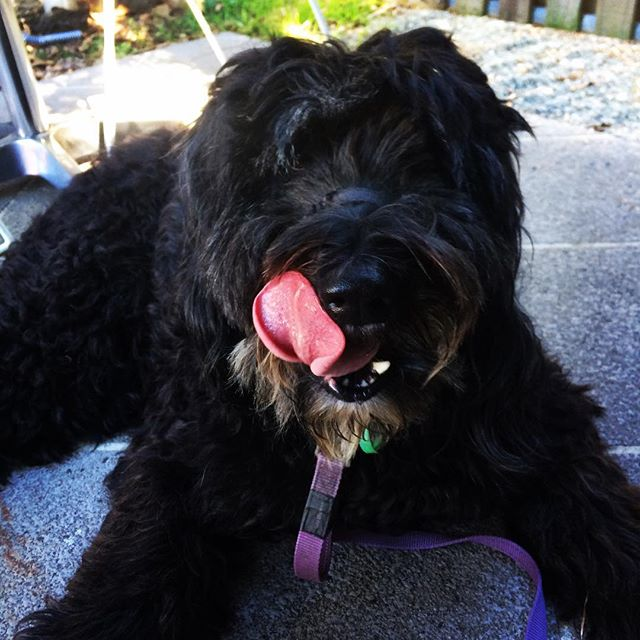
\includegraphics[width=\textwidth,keepaspectratio]{doggo2.jpg}
\end{topic}

\end{document} 
